\documentclass{article}
\usepackage{amsmath}
\usepackage{amssymb}
\usepackage{graphicx}
\usepackage{listings}
\usepackage{xcolor}
\usepackage{url} % URLを扱うために必要
\usepackage{array} % 表のための機能を追加
\usepackage{booktabs} % 表のための上下の罫線とmidruleを提供
\usepackage{multirow} % 表のセルを複数行に結合するために必要
\usepackage{subcaption} % サブフィギュアを使用するために必要
\usepackage{float} % 図の位置制御のためのパッケージを追加

% LaTeXが\midruleを認識できない問題を解決するため、booktabsを再度確認
\makeatletter
\@ifpackageloaded{booktabs}{}{\usepackage{booktabs}}
\makeatother

% 日本語環境設定 (XeLaTeX用)
\usepackage{fontspec}
\usepackage{xeCJK}
\setCJKmainfont{Hiragino Sans GB} % macOSの場合、より広範囲で利用可能なフォントに変更
\setCJKmonofont{Hiragino Sans GB} % モノスペースフォントも設定

% リスティング設定
\lstset{
    language=Matlab, % デフォルト言語をMatlabに設定
    backgroundcolor=\color{white},
    basicstyle=\ttfamily\footnotesize,
    keywordstyle=\color{blue}\bfseries,
    commentstyle=\color{green!60!black},
    stringstyle=\color{red},
    numbers=left,
    numberstyle=\tiny\color{gray},
    stepnumber=1,
    numbersep=5pt,
    frame=single,
    breaklines=true,
    showstringspaces=false,
    captionpos=b
}

\begin{document}

\title{数値解析レポート\\共役勾配法における計算精度と行列サイズの影響}
\author{学籍番号:1423107 \\ 氏名:山北倫太郎 \\ 日付:\today}
\date{}

\maketitle

\section{実験目的}
本レポートでは、大規模な連立一次方程式 $Ax=b$ の数値解法である共役勾配法(CG法)に着目し、特に計算に用いる精度(多倍長精度)と行列サイズがCG法の収束性および計算時間に与える影響について考察することを目的とする。異なる精度とサイズの行列に対するCG法の性能を比較することで、CG法における丸め誤差の影響と、大規模問題への適用可能性を探る。

\section{問題設定}
本実験では、線形連立方程式 $Ax=b$ を解くことを目的とした。ここで、$A$ は係数行列、$x$ は未知の解ベクトル、$b$ は既知の右辺ベクトルである。

\subsection{対象とする行列}
本実験では、Pythonの`mpmath`ライブラリで生成される特定の形式の行列($A_{i,j} = \text{dim} - \max(i, j)$)を用いたCG法の性能を評価した。この行列は対称行列であり、正定値性も持つように構成される。

\subsection{パラメータ設定}
\begin{itemize}
    \item \textbf{行列サイズ (dim)}: $\{500, 600, 700, 800, 900, 1000\}$ を用いた。
    \item \textbf{右辺ベクトル $b$}: 真の解 $x = [1, 2, \dots, \text{dim}]^T$ を用い、$b = Ax$ として計算した。
    \item \textbf{初期解 $x_0$}: ゼロベクトルとした。
    \item \textbf{収束判定条件}: 相対残差 $||b-Ax^{(k)}||_2 / ||b||_2 < \epsilon$ とし、$\epsilon = 10^{-15}$ と設定した。
    \item \textbf{最大反復回数}: 各行列の次元数(dim)の10倍とした。
    \item \textbf{計算精度 (dps)}: `mpmath`ライブラリにおける10進精度桁数(digits per second)を $\{30, 50, 100, 200, 500\}$ と設定し、CG法の収束に与える影響を比較した。
\end{itemize}

\section{理論}
共役勾配法(CG法)は、対称正定値行列 $A$ に対する連立一次方程式 $Ax=b$ を解くための強力な反復解法である。CG法は、二次形式の目的関数 $f(x) = \frac{1}{2}x^T Ax - x^T b$ を最小化することに基づいており、この目的関数は $Ax=b$ の解 $x$ で最小値をとる。CG法は、互いに干渉しない共役な方向 (conjugate direction) を用いて探索を行う。これにより、最急降下法と比較して、よりよい軌道で最適解に近づき、収束が速いことが理論的に知られている。

CG法の基本的なアルゴリズムは以下の通りである:
\begin{enumerate}
    \item 初期値 $x_0 \in \mathbb{R}^n$ を決める。
    \item $r_0 := b - Ax_0$, $p_0 := r_0$ とする。
    \item $k = 0, 1, 2, \dots$ に対して以下を計算する。
    \begin{itemize}
        \item (a) $\alpha_k := \frac{(r_k, p_k)}{(p_k, Ap_k)}$
        \item (b) $x_{k+1} := x_k + \alpha_k p_k$
        \item (c) $r_{k+1} := r_k - \alpha_k Ap_k$
        \item (d) $\beta_k := \frac{||r_{k+1}||_2^2}{||r_k||_2^2}$
        \item (e) 収束判定
        \item (f) $p_{k+1} := r_{k+1} + \beta_k p_k$
    \end{itemize}
\end{enumerate}

CG法は理論的には最大 $n$ 回の反復で収束する直接法と見なすことができるが、丸め誤差の影響を大きく受けるため、通常は反復法として用いられる。丸め誤差が入らないと仮定すれば、高々 $n$ 回の反復でCG法は解に収束するとされているが、実際には丸め誤差に弱いため、収束判定に基づいて反復を制御する必要がある。資料の図8.3に示されるように、多倍長精度計算を行うと、丸め誤差が小さくなるにつれて反復回数が少なくなることが明確に分かる\cite{lecture_notes}。

\section{実験結果}
提供されたPythonスクリプトを実行して得られた実験結果を表\ref{tab:results_summary}に示す。
\begin{table}[h!]
\centering
    \caption{CG法における精度(dps)と行列サイズの影響}
    \label{tab:results_summary}
    \begin{tabular}{|c|c|c|c|c|}
        \toprule
        \textbf{精度 (dps)} & \textbf{行列サイズ} & \textbf{反復回数} & \textbf{計算時間(秒)} & \textbf{相対誤差} \\
        \midrule
        \multirow{6}{*}{30} & 500 & 320 & 50.32946111 & 1.11E-15 \\
        & 600 & 371 & 78.02789879 & 1.30E-15 \\
        & 700 & 422 & 120.6168691 & 1.47E-15 \\
        & 800 & 471 & 181.2206571 & 1.86E-15 \\
        & 900 & 519 & 251.6131372 & 2.69E-15 \\
        & 1000 & 568 & 359.6314049 & 3.03E-15 \\
        \midrule
        \multirow{6}{*}{50} & 500 & 232 & 33.91785718 & 9.89E-16 \\
        & 600 & 262 & 55.24989081 & 1.95E-15 \\
        & 700 & 295 & 90.14068413 & 2.43E-15 \\
        & 800 & 326 & 126.5693463 & 3.17E-15 \\
        & 900 & 362 & 185.4492209 & 3.13E-15 \\
        & 1000 & 388 & 237.0105391 & 3.87E-15 \\
        \midrule
        \multirow{6}{*}{100} & 500 & 164 & 23.98174596 & 1.03E-15 \\
        & 600 & 187 & 39.36424613 & 1.52E-15 \\
        & 700 & 206 & 61.25863292 & 2.10E-15 \\
        & 800 & 225 & 88.77976489 & 3.13E-15 \\
        & 900 & 242 & 122.2011493 & 3.47E-15 \\
        & 1000 & 261 & 165.6940129 & 4.49E-15 \\
        \midrule
        \multirow{6}{*}{200} & 500 & 136 & 20.50235821 & 1.21E-15 \\
        & 600 & 150 & 34.08881402 & 1.86E-15 \\
        & 700 & 164 & 51.65259504 & 2.71E-15 \\
        & 800 & 178 & 71.61412573 & 2.74E-15 \\
        & 900 & 189 & 97.42211199 & 4.62E-15 \\
        & 1000 & 203 & 131.7460811 & 4.32E-15 \\
        \midrule
        \multirow{6}{*}{500} & 500 & 126 & 20.96529269 & 1.22E-15 \\
        & 600 & 137 & 35.03951406 & 1.90E-15 \\
        & 700 & 147 & 60.21019411 & 2.77E-15 \\
        & 800 & 158 & 93.23292613 & 2.83E-15 \\
        & 900 & 167 & 118.3835537 & 3.31E-15 \\
        & 1000 & 176 & 150.7689443 & 4.52E-15 \\
        \bottomrule
    \end{tabular}
\end{table}

\subsection{グラフ}
以下の図に、実験結果を視覚化したグラフを示す。

% 図1: [H]で強制的にここに配置
\begin{figure}[H]
    \centering
    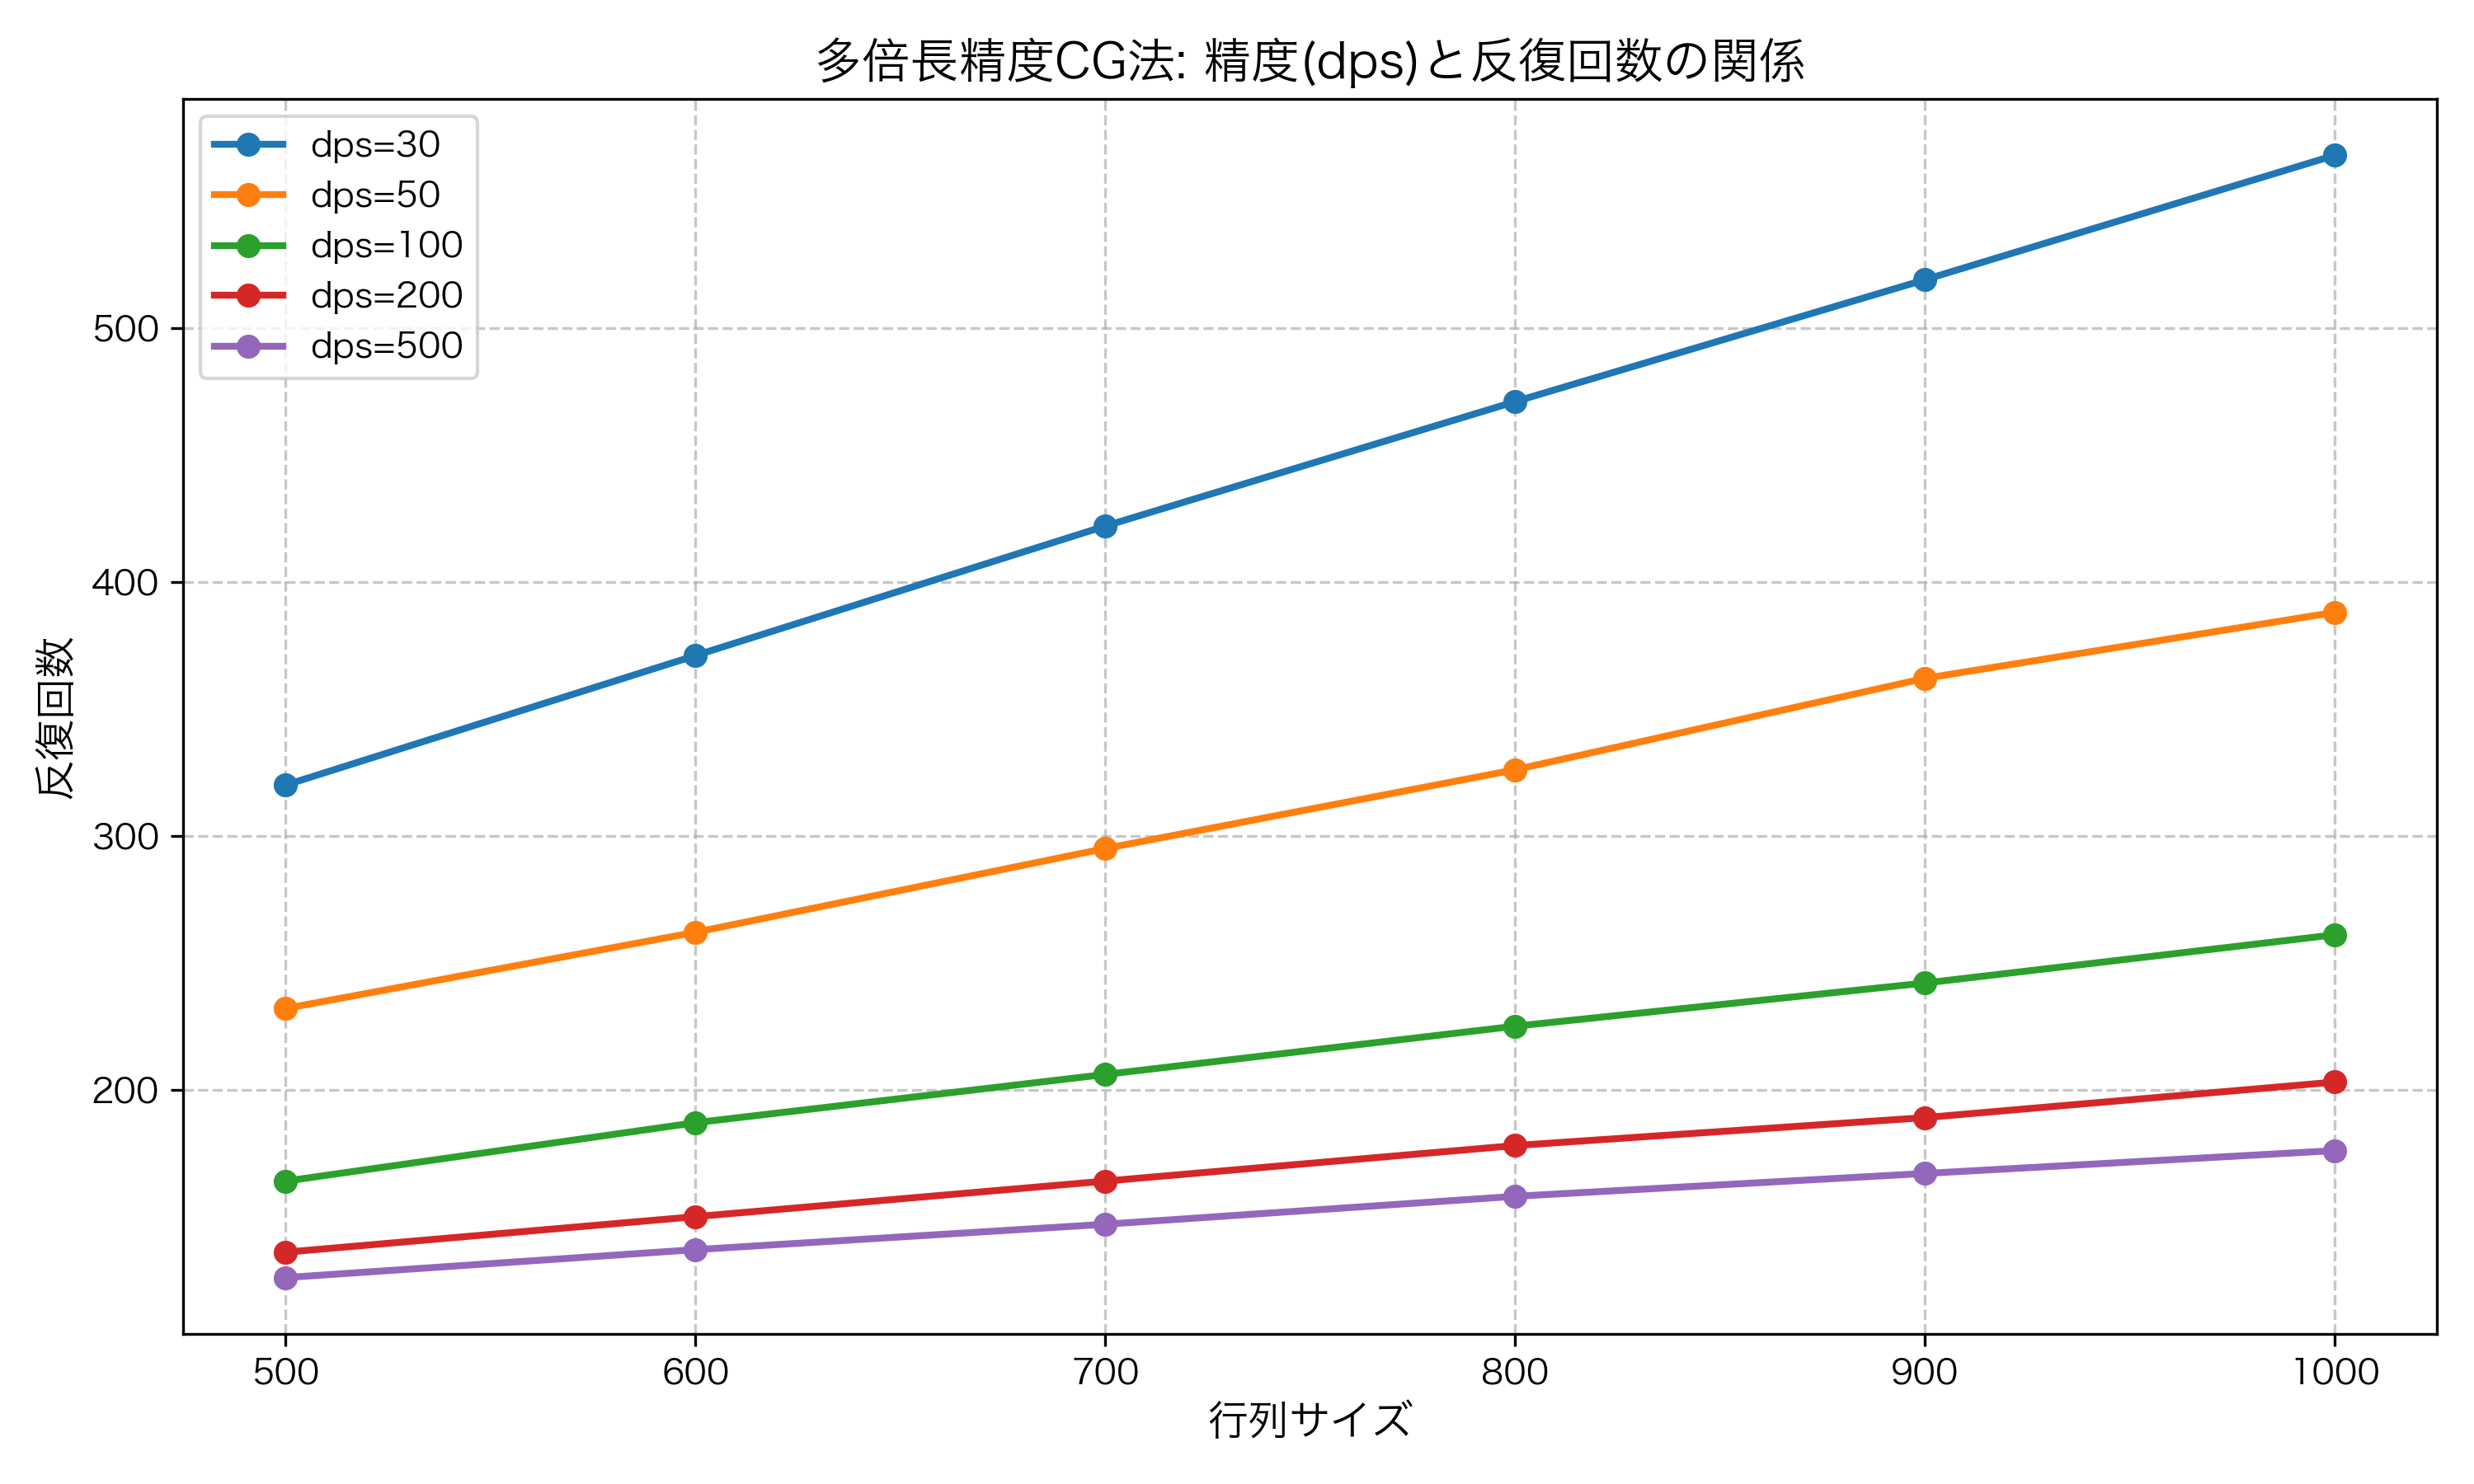
\includegraphics[width=0.8\textwidth]{mpmath_iterations_plot.png}
    \caption{反復回数と行列サイズの関係(dps別)}
    \label{fig:iterations_vs_dim}
\end{figure}

% 図2: [H]で強制的にここに配置
\begin{figure}[H]
    \centering
    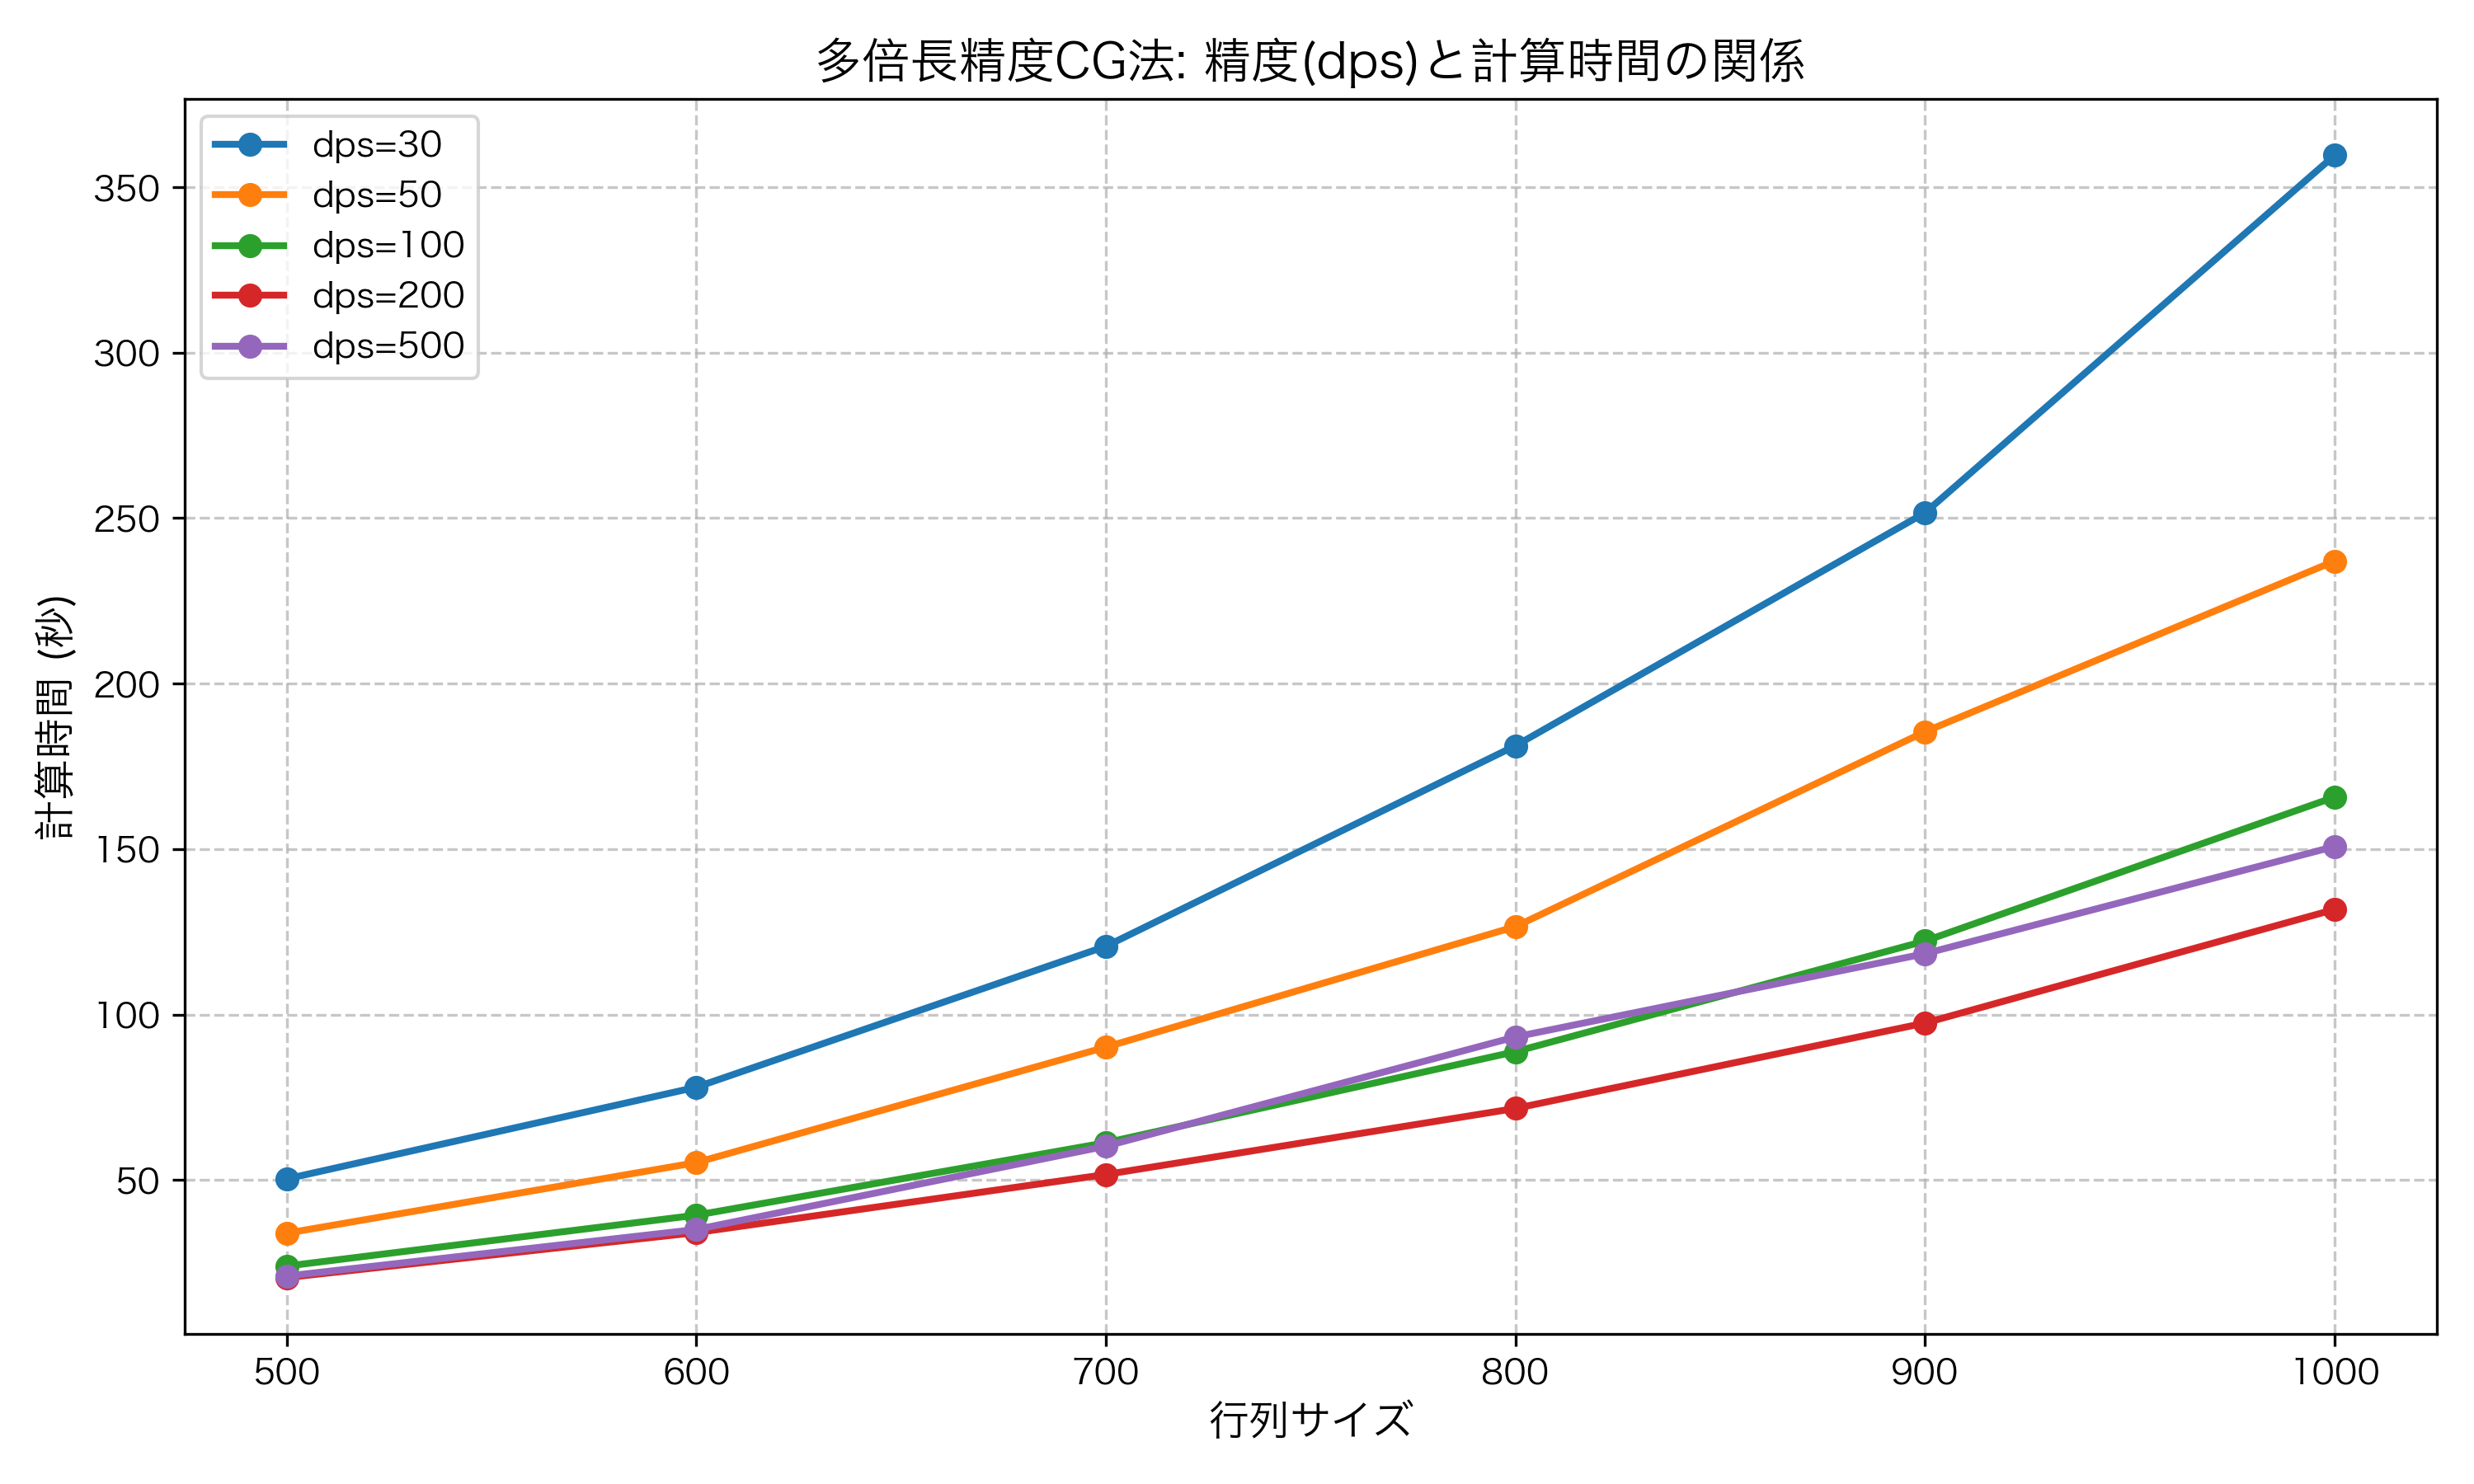
\includegraphics[width=0.8\textwidth]{mpmath_time_plot.png}
    \caption{計算時間と行列サイズの関係(dps別)}
    \label{fig:time_vs_dim}
\end{figure}

% 図3: [H]で強制的にここに配置
\begin{figure}[H]
    \centering
    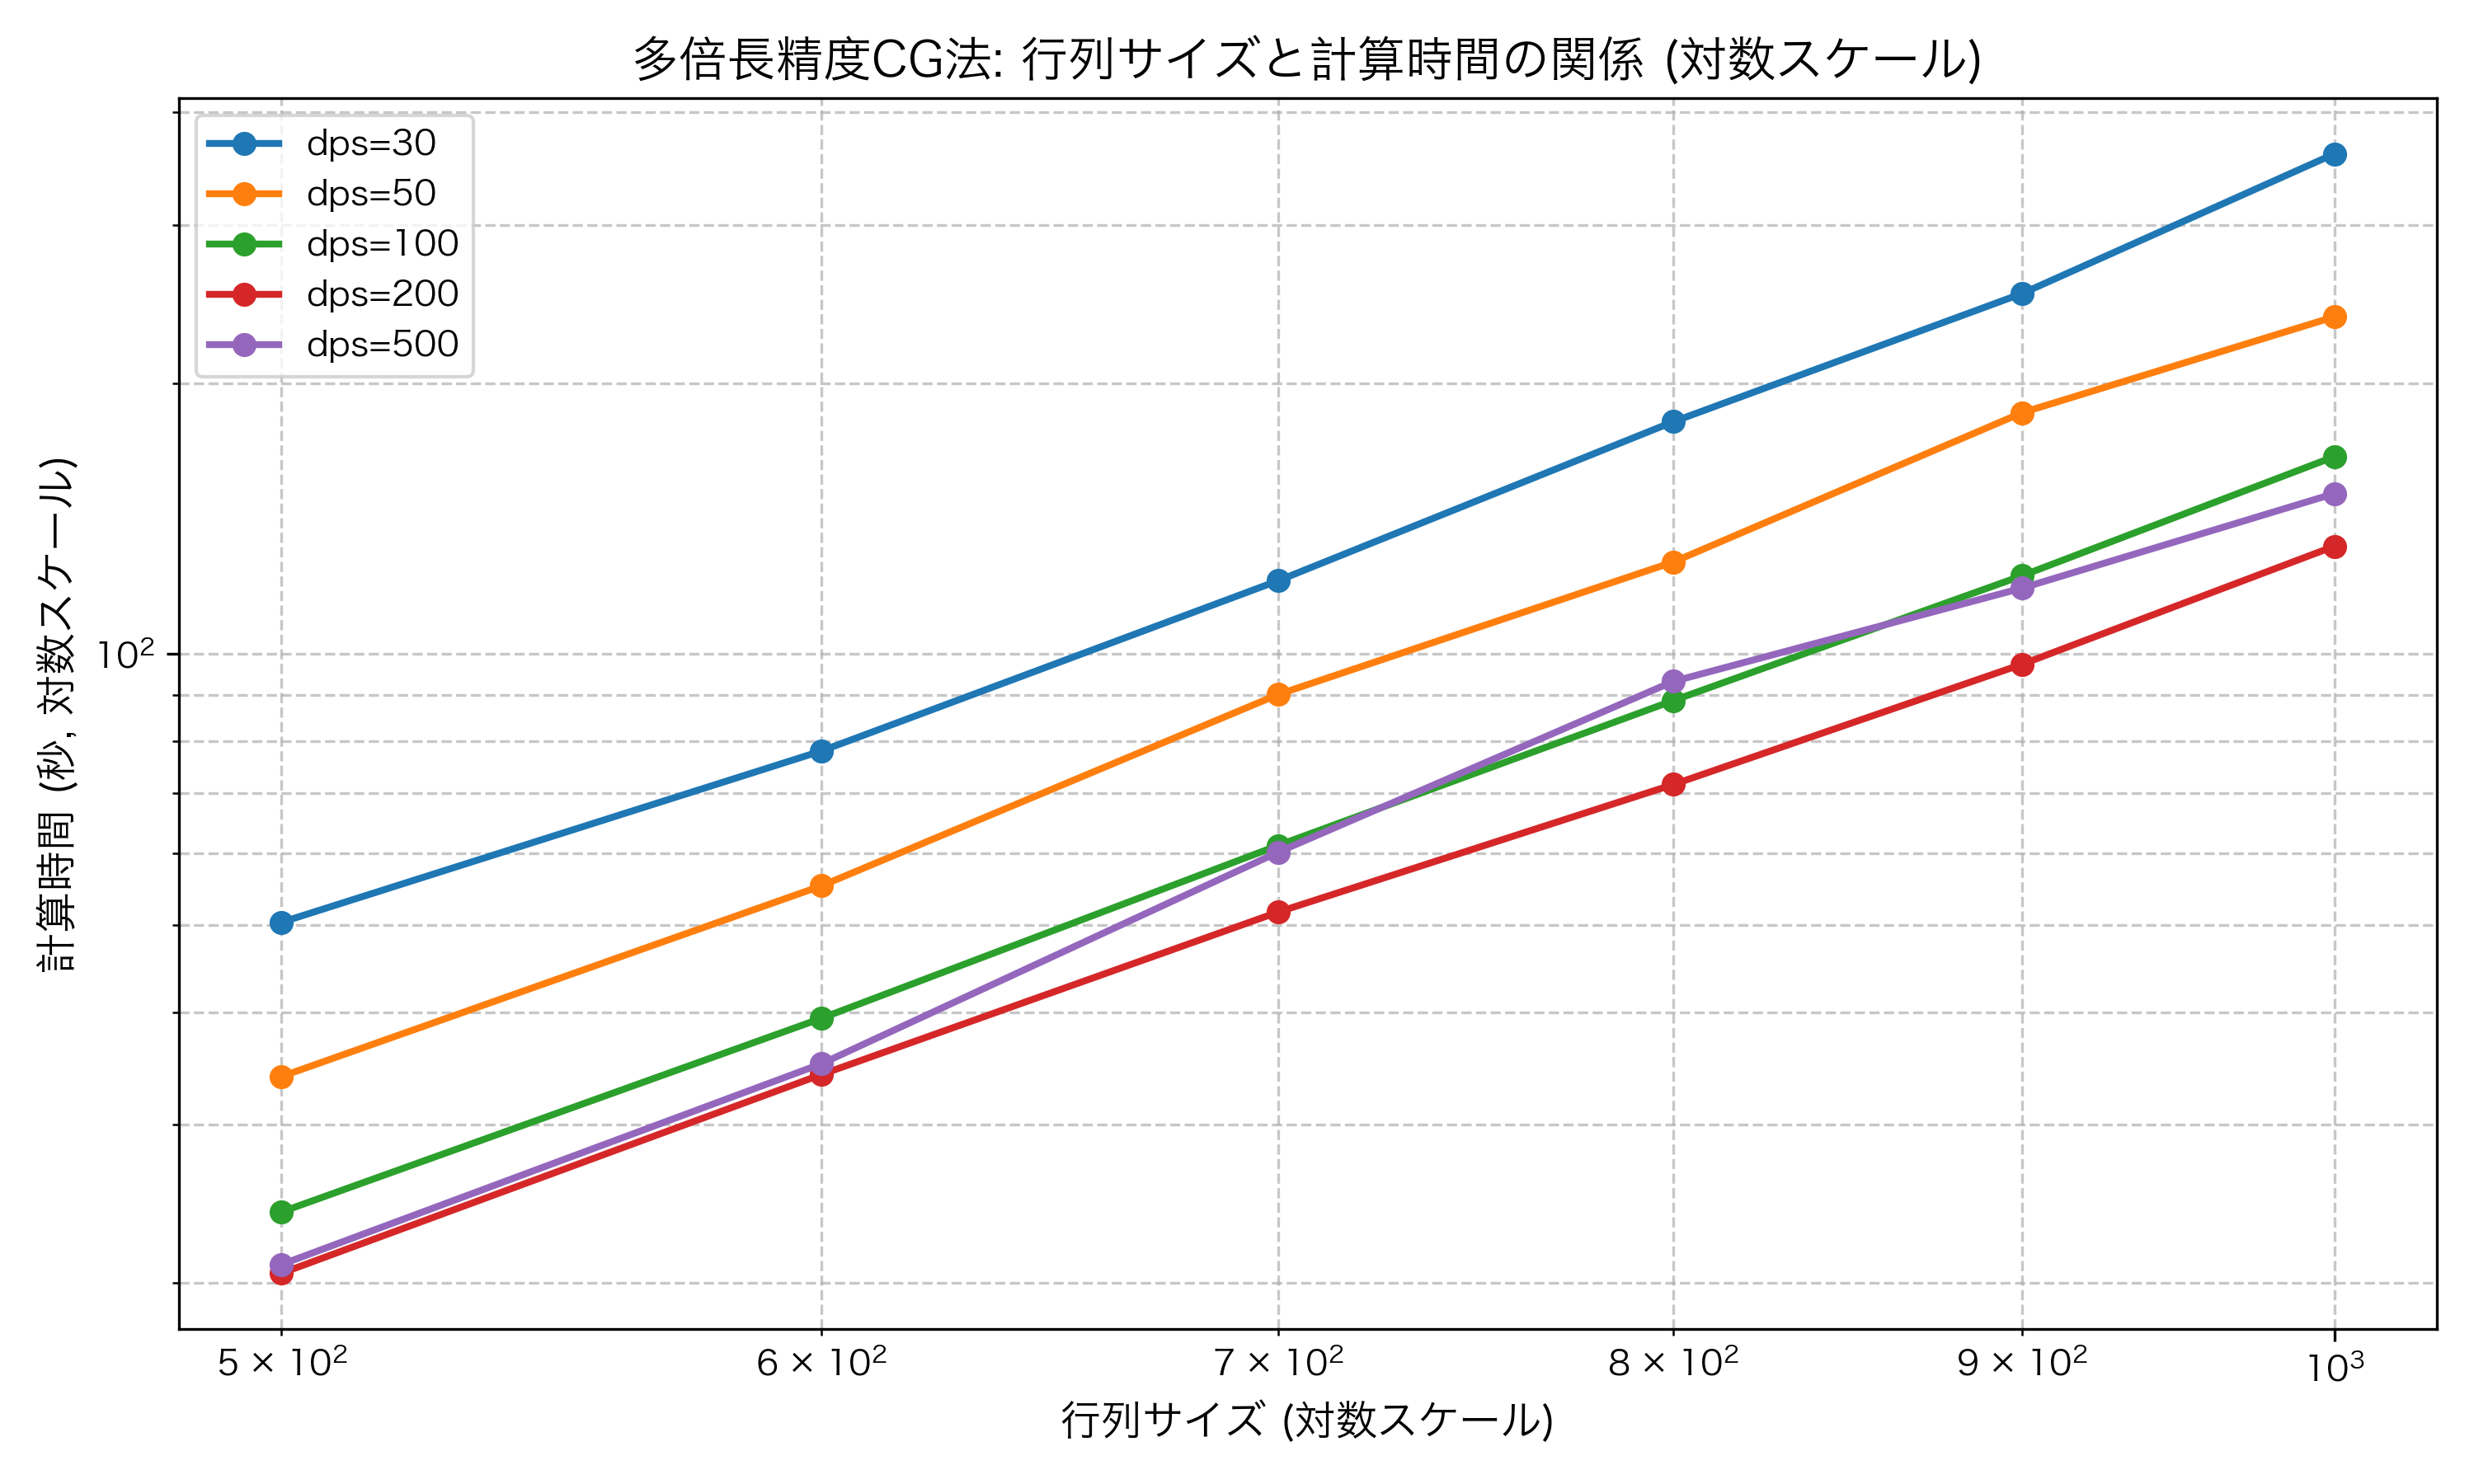
\includegraphics[width=0.8\textwidth]{mpmath_time_loglog_plot.png}
    \caption{計算時間と行列サイズの関係(両対数プロット)}
    \label{fig:time_loglog_plot}
\end{figure}

% 図4: [H]で強制的にここに配置(サブフィギュア)
\begin{figure}[H]
    \centering
    \begin{subfigure}[b]{0.48\textwidth}
        \centering
        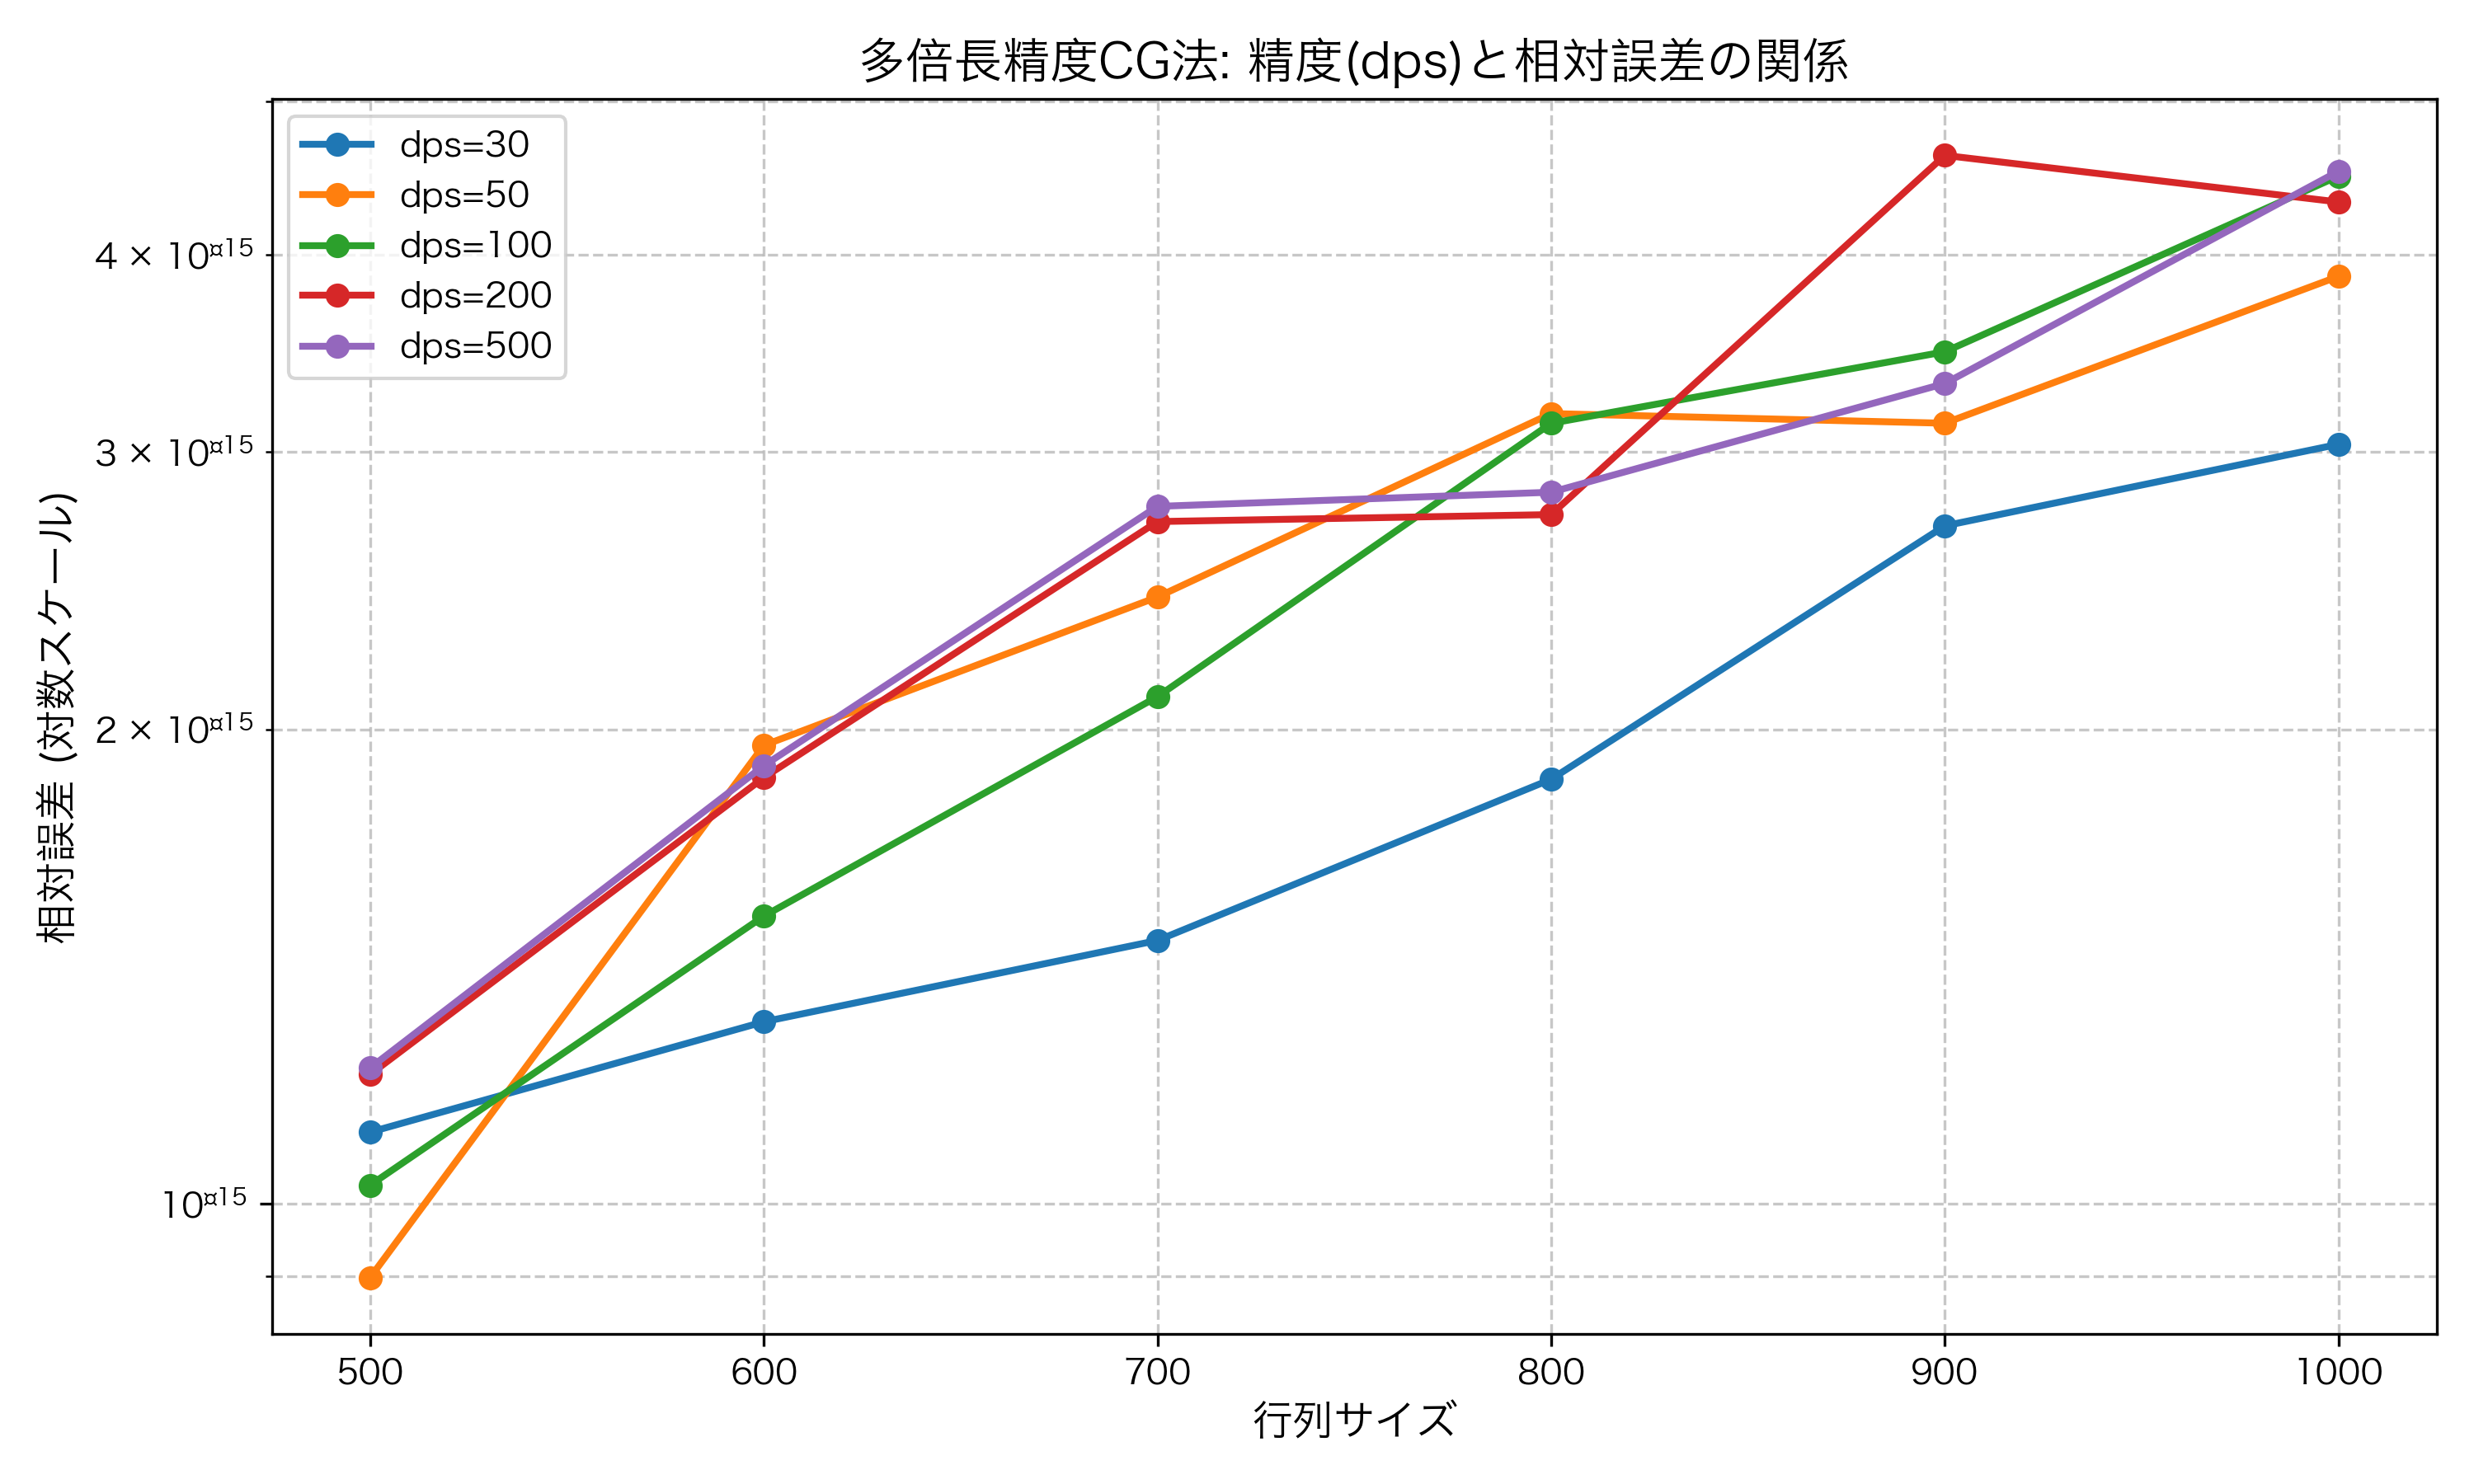
\includegraphics[width=\textwidth]{mpmath_error_plot.png}
        \caption{相対誤差と行列サイズの関係(dps別)}
        \label{fig:error_vs_dim}
    \end{subfigure}
    \hfill
    \begin{subfigure}[b]{0.48\textwidth}
        \centering
        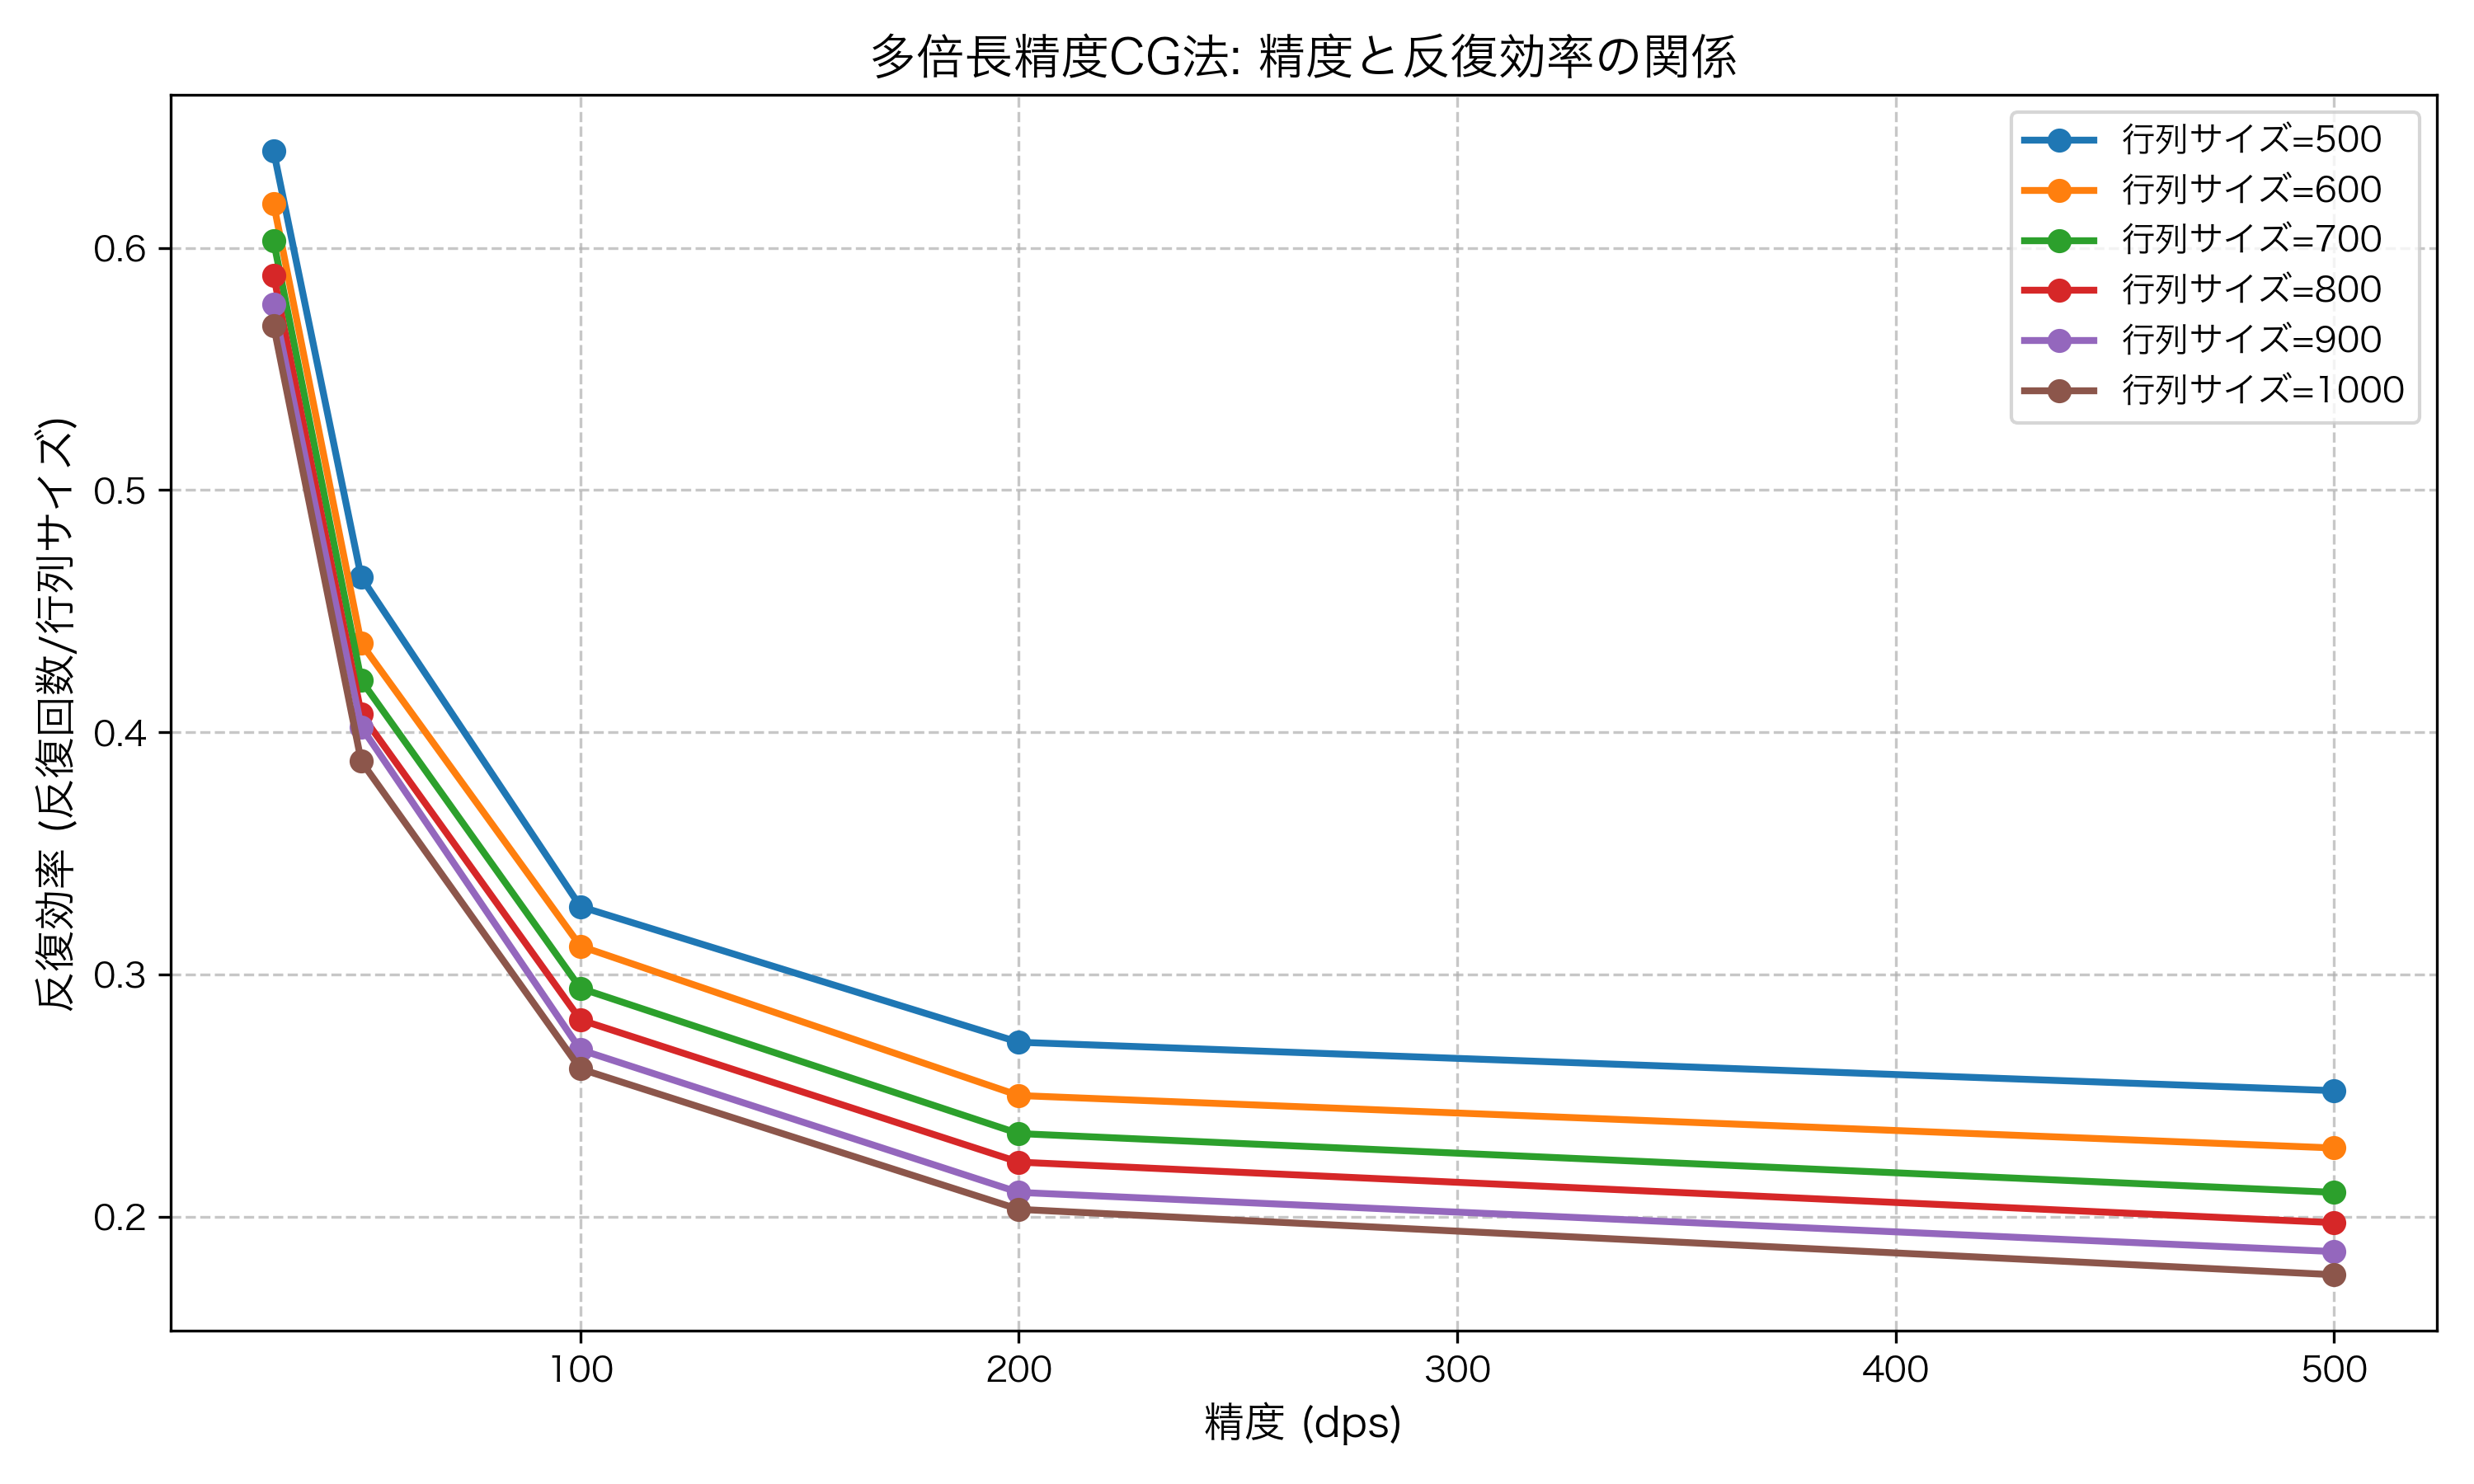
\includegraphics[width=\textwidth]{mpmath_efficiency_plot.png}
        \caption{反復回数/行列サイズ(効率性)と行列サイズの関係(dps別)}
        \label{fig:efficiency_vs_dim}
    \end{subfigure}
    \caption{誤差と効率性の分析}
    \label{fig:error_efficiency}
\end{figure}

% 図5: [H]で強制的にここに配置
\begin{figure}[H]
    \centering
    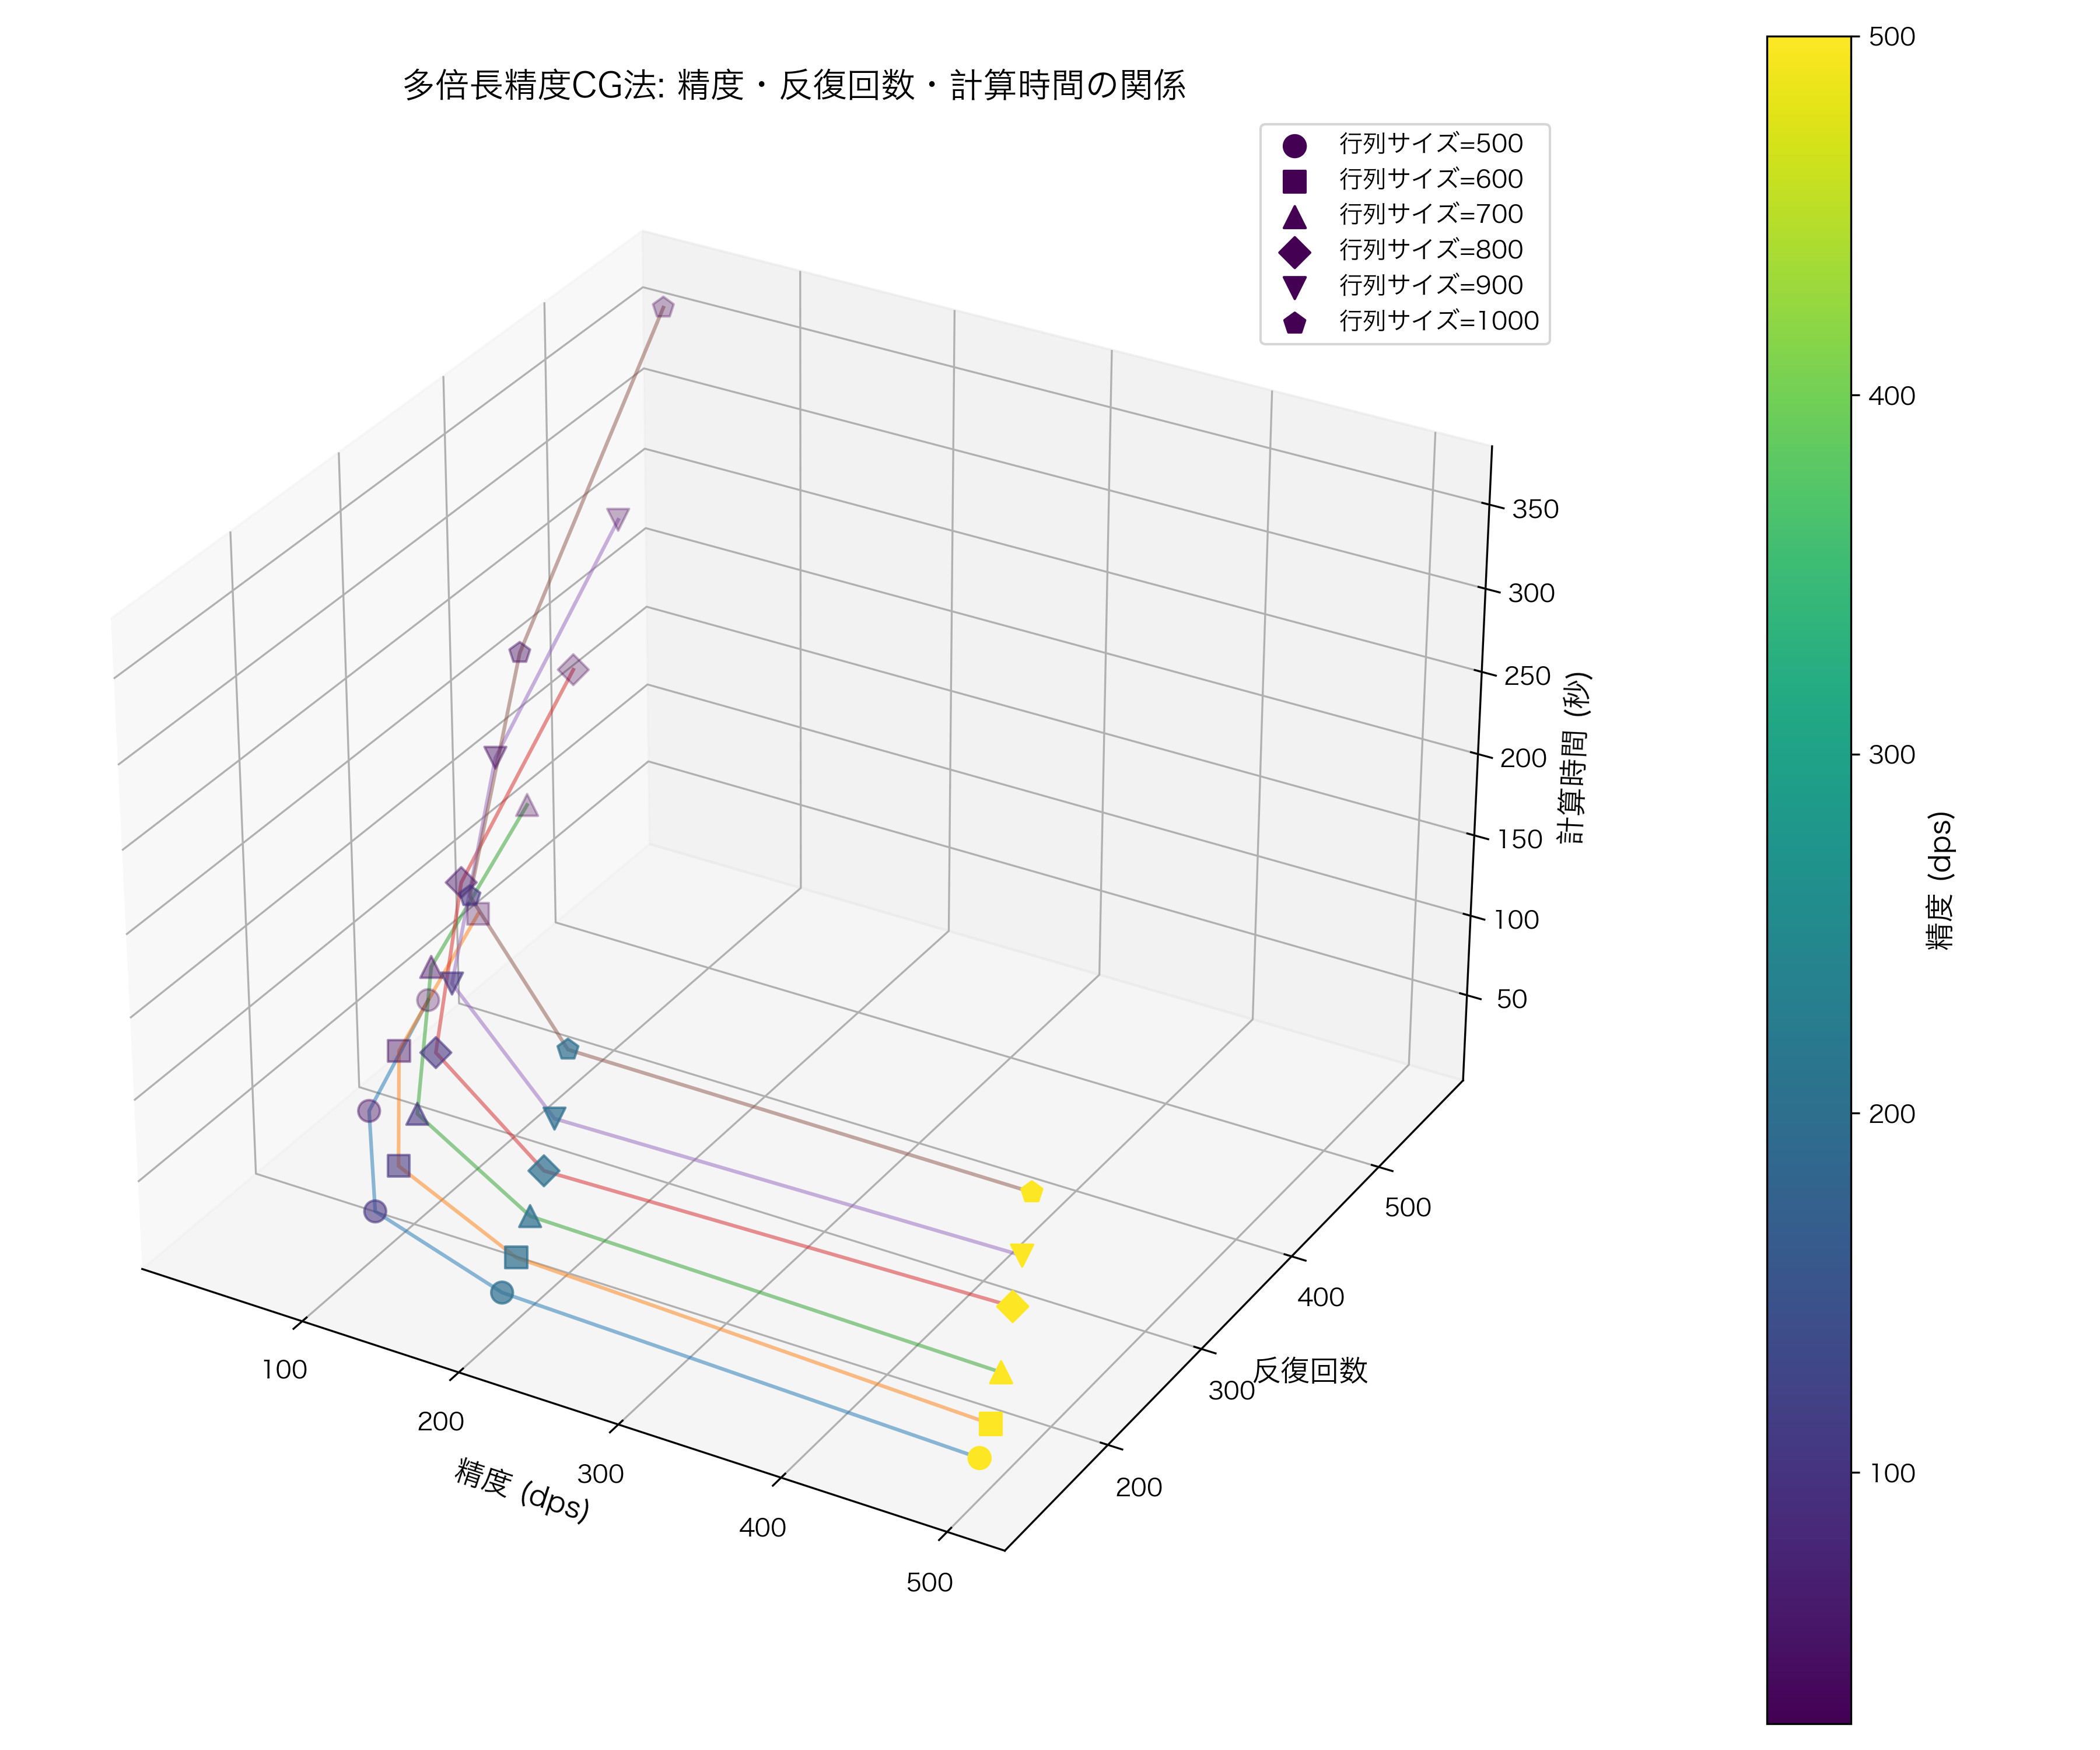
\includegraphics[width=0.8\textwidth]{mpmath_3d_plot.png}
    \caption{行列サイズ・精度(dps)・計算時間の3次元関係}
    \label{fig:3d_plot}
\end{figure}
\section{考察}

\subsection{計算精度 (dps) の影響}
表1および図\ref{fig:iterations_vs_dim}から、CG法の収束性において、計算精度(dps)が極めて重要な役割を果たすことが明確に示された。dpsの値が増加するにつれて、CG法が要求される相対誤差の基準($10^{-15}$)を満たすために必要な反復回数が著しく減少している。例えば、行列サイズ500の場合、dps=30では320回であった反復回数が、dps=500では126回にまで減少している。これは、より高い精度で計算を行うことで、丸め誤差の影響が抑制され、CG法の理論的な収束特性がより顕著に現れるためである。相対誤差はすべてのdpsと行列サイズで$10^{-15}$のオーダーに達しており、設定した収束基準を満たしている(図\ref{fig:error_vs_dim})。

計算時間については(図\ref{fig:time_vs_dim}、図\ref{fig:time_loglog_plot})、反復回数の減少に伴い、計算時間も減少する傾向が見られる。しかし、dpsを高くすると、1回あたりの浮動小数点演算にかかるコストが増加するため、反復回数が大幅に減っても計算時間の減少が比例しない場合がある。例えば、dps=200とdps=500を比較すると、反復回数は減少しているものの、計算時間の減少幅は小さくなっている、あるいはわずかに増加しているケースもある。これは、多倍長精度計算のオーバヘッドが効いてくるためと考えられる。最も効率の良い精度は、問題の性質と計算機の性能に依存すると考えられる。

\subsection{行列サイズの影響}
各dps設定において、行列サイズが増加するにつれて、反復回数および計算時間が増加する傾向が確認された(図\ref{fig:iterations_vs_dim}、図\ref{fig:time_vs_dim})。反復回数は行列サイズにほぼ比例して増加しており、これはCG法の反復回数が問題の次元に依存するという理論的な側面と一致する。計算時間も同様に行列サイズの増加に伴い増加しているが、その増加率はdpsの値によって異なる傾向が見られる。特に図\ref{fig:time_loglog_plot}の両対数プロットからは、計算時間が次元に対してほぼ線形に増加していることが示唆される。

図\ref{fig:efficiency_vs_dim}では、反復回数を行列サイズで割った値(効率性の指標)が示されており、dpsが高いほどこの値が低い、すなわちより少ない反復で行列サイズに対する問題を解けていることが分かる。これは、高精度計算が高次元問題に対するCG法の効率を向上させる可能性を示している。

\subsection{丸め誤差の影響}
今回の実験では、`mpmath`ライブラリを用いて非常に高い精度(dps=500では$10^{-15}$以上の相対誤差を達成)で計算が行われているため、通常の倍精度浮動小数点演算では無視できない丸め誤差の影響が大幅に軽減されている。この結果は、丸め誤差がCG法の収束を阻害する主要因であることを改めて示している。特に、より低いdps設定(例:dps=30, 50)では、反復回数が多くなる傾向があり、これは丸め誤差の影響が比較的大きいことを示唆する。図\ref{fig:3d_plot}は、計算時間が行列サイズとdpsの両方に依存し、高dpsでは反復回数が減るものの、1反復あたりのコストが増加するというトレードオフを視覚的に示している。

\section{結論}
本レポートにおける数値実験により、共役勾配法(CG法)において、計算精度(dps)と行列サイズがその性能に重要な影響を与えることが実証された。計算精度を向上させることで、CG法の収束に必要な反復回数を大幅に削減できることが明らかになった。これは、CG法が丸め誤差に敏感であるという理論的な性質を裏付けるものである。

一方で、計算精度を高めると1回あたりの演算コストが増加するため、最も効率的な計算精度は問題と計算環境によって異なることが示唆された。行列サイズが増加すると反復回数および計算時間が増加するが、適切な精度設定により、大規模な問題に対しても高い精度で効率的に解を得られることが示された。

今後の課題としては、この特定の行列形式だけでなく、より多様な大規模疎行列に対するCG法の性能評価を行うことが挙げられる。また、前処理付き共役勾配法(PCG法)を多倍長精度計算に適用した場合の性能向上についても検討する価値がある。

\section{感想}
今回のレポート作成を通じて、数値計算における「精度」という概念が、単なる理論的な話ではなく、実際のアルゴリズムの性能に直結する非常に実践的な要素であることを深く理解することができました。特に、多倍長精度計算を用いることで、丸め誤差という普段意識しにくい要素がCG法の収束にどれほど大きな影響を与えているのかを数値とグラフで確認できたことは、非常に興味深い経験でした。行列サイズが大きくなるにつれて計算時間が指数関数的に増大していく中で、限られた計算リソースの中でいかに最適な精度と次元を選択するかという課題の奥深さを感じました。

\section{参考文献}
\begin{thebibliography}{9}
\bibitem{source: 1} 工学博士 田中敏幸. \textit{数値計算法基礎}.
\bibitem{source: 2} 幸谷智紀. \textit{Python数値計算プログラミング}.
\bibitem{source: 3} 洲之内治男, 石渡恵美子. \textit{数値計算 新訂版}.
\end{thebibliography}

\section{付録: プログラムコード}
\subsection{cg\_experiment.py}
\begin{lstlisting}[language=Python, caption=cg\_experiment.py]

# filepath: /Users/rintaro/Downloads/Github_private/machine_learning/ConjugateGradientMethodreport/cg_experiment.py
import numpy as np
import time
import csv
import os
import mpmath
import mpmath.libmp
from datetime import datetime

# CG法(mpmath版)
def cg(vec_x, mat_a, vec_b, rtol, atol, max_times):
    dim = vec_x.rows
    r = vec_b - mat_a * vec_x
    p = r
    rsold = (r.T * r)[0, 0]

    init_norm_r = mpmath.norm(r)
    old_norm_r = init_norm_r
    
    for times in range(max_times):
        ap = mat_a * p
        
        alpha = rsold / (p.T * ap)[0, 0]
        
        vec_x = vec_x + alpha * p
        r = r - alpha * ap
        rsnew = (r.T * r)[0, 0]

        # 残差ノルムの更新
        new_norm_r = mpmath.norm(r)
        
        # 収束判定
        if new_norm_r <= (rtol * init_norm_r + atol):
            break
        
        beta = rsnew / rsold
        p = r + beta * p
        rsold = rsnew
        
    return times + 1, vec_x  # 反復回数は0から始まるので+1

def run_experiment(dps_values, dim_values):
    # 結果を保存するためのリスト
    results = []
    
    # 実験日時を取得
    now = datetime.now()
    date_str = now.strftime("%Y%m%d_%H%M%S")
    
    # ファイル名の設定
    csv_filename = f'cg_experiment_results_{date_str}.csv'
    txt_filename = f'cg_experiment_results_{date_str}.txt'
    
    # テキストファイルに実験情報を書き込み
    with open(txt_filename, 'w') as txtfile:
        txtfile.write("共役勾配法の精度と行列サイズに関する実験結果\n")
        txtfile.write(f"実験日時: {now.strftime('%Y年%m月%d日 %H:%M:%S')}\n\n")
        txtfile.write(f"使用する精度: {dps_values}\n")
        txtfile.write(f"使用する行列サイズ: {dim_values}\n\n")
        txtfile.write(f"実験開始: {len(dps_values) * len(dim_values)}回の実験を実行します\n\n")
    
    # CSVのヘッダー
    header = ['精度(dps)', '行列サイズ', '反復回数', '計算時間(秒)', '相対誤差']
    
    print(f"実験開始: {len(dps_values) * len(dim_values)}回の実験を実行します")
    
    # 各精度と行列サイズの組み合わせで実験
    for dps in dps_values:
        mpmath.mp.dps = dps
        print(f"\n10進精度桁数 = {mpmath.mp.dps}")
        
        # テキストファイルに記録
        with open(txt_filename, 'a') as txtfile:
            txtfile.write(f"\n10進精度桁数 = {mpmath.mp.dps}\n")
        
        for dim in dim_values:
            print(f"正方行列サイズ dim = {dim} の実験を開始...")
            
            # 行列要素を設定
            mat_a = mpmath.zeros(dim, dim)
            for i in range(dim):
                for j in range(dim):
                    mat_a[i, j] = mpmath.mpf(dim - max(i, j))
            
            # x = [1, 2, ..., dim] の真の解を生成
            vec_true_x = mpmath.matrix([mpmath.mpf(i) for i in range(1, dim + 1)])
            
            # b = A * x を計算
            vec_b = mat_a * vec_true_x

            # CG法実行
            vec_x = mpmath.zeros(dim, 1)  # 初期解をゼロベクトルに設定
            
            start_time = time.time()
            iterative_times, vec_x = cg(vec_x, mat_a, vec_b, 2.00e-20, 0.0, dim * 10)
            time_taken = time.time() - start_time
            
            # 相対誤差の計算
            relerr = mpmath.norm(vec_x - vec_true_x) / mpmath.norm(vec_true_x)
            
            # 結果の表示
            result_str = f'CG: 反復回数={iterative_times}, 時間={time_taken:.4f}秒, 相対誤差={mpmath.nstr(relerr)}'
            print(result_str)
            
            # テキストファイルに記録
            with open(txt_filename, 'a') as txtfile:
                txtfile.write(f"正方行列サイズ dim = {dim}\n")
                txtfile.write(f"{result_str}\n\n")
            
            # 結果をリストに追加
            results.append([dps, dim, iterative_times, time_taken, float(relerr)])
    
    # 結果をCSVファイルに保存
    with open(csv_filename, 'w', newline='') as csvfile:
        writer = csv.writer(csvfile)
        writer.writerow(header)
        writer.writerows(results)
    
    # 結果の要約をテキストファイルに追加
    with open(txt_filename, 'a') as txtfile:
        txtfile.write("\n\n実験結果の要約:\n")
        txtfile.write("精度(dps) | 行列サイズ | 反復回数 | 計算時間(秒) | 相対誤差\n")
        txtfile.write("-" * 70 + "\n")
        
        for result in results:
            summary_line = f"{result[0]:<10} | {result[1]:<10} | {result[2]:<8} | {result[3]:<12.4f} | {result[4]:.4e}"
            txtfile.write(summary_line + "\n")
    
    print(f"\n実験完了!結果は以下のファイルに保存されました:")
    print(f"CSVファイル: {csv_filename}")
    print(f"テキストファイル: {txt_filename}")
    
    return results

if __name__ == '__main__':
    # 実験パラメータ
    dps_values = [30, 50, 100, 200, 500]
    dim_values = [500, 600, 700, 800, 900, 1000]
    
    print("共役勾配法の精度と行列サイズに関する実験")
    print(f"使用する精度: {dps_values}")
    print(f"使用する行列サイズ: {dim_values}")
    
    # 実験の実行
    results = run_experiment(dps_values, dim_values)
    
    # 結果の要約
    print("\n実験結果の要約:")
    print("精度(dps) | 行列サイズ | 反復回数 | 計算時間(秒) | 相対誤差")
    print("-" * 70)
    
    for result in results:
        print(f"{result[0]:<10} | {result[1]:<10} | {result[2]:<8} | {result[3]:<12.4f} | {result[4]:.4e}")
\end{lstlisting}

\subsection{cg\_mpmath.py}
\begin{lstlisting}[language=Python, caption=cg\_mpmath.py]
# filepath: /Users/rintaro/Downloads/Github_private/machine_learning/ConjugateGradientMethodreport/cg_mpmath.py
import numpy as np
import time

# cg_mpmath.py: 多倍長精度CG法 
import mpmath  # 多倍長精度計算
import mpmath.libmp  # 可能ならばgmpy2を使用

# 計算精度初期設定
mpmath.mp.dps = 30  # 10進精度桁数
input_dps = input('10進精度桁数 dps (推奨: 30, 50, 100, 200, 500): ')
if int(input_dps) > mpmath.mp.dps:
    mpmath.mp.dps = int(input_dps)
print(f'10進精度桁数 = {mpmath.mp.dps}')

# CG法(mpmath版)
def cg(vec_x, mat_a, vec_b, rtol, atol, max_times):
    dim = vec_x.rows
    r = vec_b - mat_a * vec_x
    p = r
    rsold = (r.T * r)[0, 0]  # 内積計算を修正

    init_norm_r = mpmath.norm(r)
    old_norm_r = init_norm_r

    print("CG: iteration, time=, relerr(vec_x)=, relerr(vec_b)=, norm_r_rel")  # 追加情報
    
    for times in range(max_times):
        ap = mat_a * p
        
        # 内積計算を修正
        alpha = rsold / (p.T * ap)[0, 0]
        
        vec_x = vec_x + alpha * p
        r = r - alpha * ap
        rsnew = (r.T * r)[0, 0]  # 内積計算を修正

        # 残差ノルムの更新
        new_norm_r = mpmath.norm(r)
        
        # 収束判定
        if new_norm_r <= (rtol * init_norm_r + atol):
            break
        
        beta = rsnew / rsold
        p = r + beta * p
        rsold = rsnew
        
    return times + 1, vec_x  # 反復回数は0から始まるので+1

# メイン実行部分
if __name__ == '__main__':
    str_dim = input('正方行列サイズ dim = ')
    dim = int(str_dim)

    # 行列要素を設定
    mat_a = mpmath.zeros(dim, dim)
    for i in range(dim):
        for j in range(dim):
            mat_a[i, j] = mpmath.mpf(dim - max(i, j))
    
    # x = [1, 2, ..., dim] の真の解を生成
    vec_true_x = mpmath.matrix([mpmath.mpf(i) for i in range(1, dim + 1)])
    
    # b = A * x を計算
    vec_b = mat_a * vec_true_x

    # CG法実行
    vec_x = mpmath.zeros(dim, 1)  # 初期解をゼロベクトルに設定
    
    start_time = time.time()
    # rtol, atolは資料から2.00-20, 0.0と読み取れる
    iterative_times, vec_x = cg(vec_x, mat_a, vec_b, 2.00e-20, 0.0, dim * 10)
    time_taken = time.time() - start_time
    
    # 相対誤差の計算
    relerr = mpmath.norm(vec_x - vec_true_x) / mpmath.norm(vec_true_x)
    
    print(f'CG: iteration={iterative_times}, time={time_taken:.4f}s')
    print(f'relerr(vec_x)={mpmath.nstr(relerr)}')
\end{lstlisting}

\end{document}